%%%%%%%%%%%%%%%%%%%%%%%%%%%%%%%%%%%%%%%%%
% Cleese Assignment (For Students)
% LaTeX Template
% Version 2.0 (27/5/2018)
%
% This template originates from:
% http://www.LaTeXTemplates.com
%
% Author:
% Vel (vel@LaTeXTemplates.com)
%
% License:
% CC BY-NC-SA 3.0 (http://creativecommons.org/licenses/by-nc-sa/3.0/)
% 
%%%%%%%%%%%%%%%%%%%%%%%%%%%%%%%%%%%%%%%%%

%----------------------------------------------------------------------------------------
%	PACKAGES AND OTHER DOCUMENT CONFIGURATIONS
%----------------------------------------------------------------------------------------

\documentclass[fleqn]{article}
\usepackage{float}
\usepackage{amsmath, amssymb}
\usepackage{amsmath}
\usepackage{mathtools}
\usepackage{graphicx}
\usepackage{amsmath}
\usepackage{mathrsfs,amsmath}
\DeclareMathOperator{\sinc}{sinc}
%\usepackage[printwatermark]{xwatermark}
%\newwatermark[allpages,color=gray!50,angle=45,scale=2.5,xpos=-5,ypos=-5]{Mohammad Hadi}

\input{structure.tex} % Include the file specifying the document structure and custom commands

%----------------------------------------------------------------------------------------
%	ASSIGNMENT INFORMATION
%----------------------------------------------------------------------------------------

% Required
\newcommand{\assignmentQuestionName}{Question} % The word to be used as a prefix to question numbers; example alternatives: Problem, Exercise
\newcommand{\assignmentClass}{Communication Systems (Taught by Mohammad Hadi)\\Assignment 2 (Due on DDD.,\ mmm.\ dd,\ yyyy)} % Course (Lecturer)\\Assignment (Due date)
\newcommand{\assignmentTitle}{} % Assignment title or name
\newcommand{\assignmentAuthorName}{Student Name\\Student Number} % Student name\\Student number
%----------------------------------------------------------------------------------------

\begin{document}

%----------------------------------------------------------------------------------------
%	TITLE PAGE
%----------------------------------------------------------------------------------------

\assignmentSection{Mathematical Questions}

%----------------------------------------------------------------------------------------
%	QUESTION 1
%----------------------------------------------------------------------------------------

\begin{question}
\questiontext{Calculate the power content of the SSB signal 
$
u(t) = A_c m(t)\cos(2\pi f_c t)\mp A_c \hat{m}(t)\sin(2\pi f_c t)
$.
}

\answer{

\[ P_{u}=\lim_{T \to \infty} \frac{1}{T} \int_{-\frac{T}{2}}^{+\frac{T}{2}} |u(t)|^2 \,dt \]
\[ = \lim_{T \to \infty} \frac{1}{T} \int_{-\frac{T}{2}}^{+\frac{T}{2}} [ A_c m(t)\cos(2\pi f_c t)\mp A_c \hat{m}(t)\sin(2\pi f_c t) ]^2  \,dt \] 
\[ = \lim_{T \to \infty} \frac{A_{c}^{2}}{T} \int_{-\frac{T}{2}}^{+\frac{T}{2}} [ m(t)^{2}\cos^{2}(2\pi f_{c}t) + \hat{m}(t)^{2}\sin^{2}(2\pi f_c t) \mp 2m(t)\hat{m}(t)\cos(2\pi f_{c}t)\sin(2\pi f_{c}t)] \,dt \] \\
Now we use trigonometric identities to simplify the equation:\\
\[ = \lim_{T \to \infty} \frac{A_{c}^{2}}{T} \int_{-\frac{T}{2}}^{+\frac{T}{2}} [ m(t)^{2}\frac{1+\cos(4\pi f_{c}t)}{2} + \hat{m}(t)^{2}\frac{1-\cos(4\pi f_{c}t)}{2} \mp m(t)\hat{m}(t)\sin(4\pi f_{c}t)] \,dt \] 
\[ = \lim_{T \to \infty} \frac{A_{c}^{2}}{2T}\left(\int_{-\frac{T}{2}}^{+\frac{T}{2}} m(t)^{2}\,dt + \int_{-\frac{T}{2}}^{+\frac{T}{2}} \hat{m}(t)^{2}\,dt \right) \] 
\[+ \lim_{T \to \infty} \frac{A_{c}^{2}}{2T}\left(\int_{-\frac{T}{2}}^{+\frac{T}{2}} m(t)^{2}\cos(4\pi f_{c}t) \,dt - \int_{-\frac{T}{2}}^{+\frac{T}{2}} \hat{m}(t)^{2}\cos(4\pi f_{c}t) \,dt \right) \]
\[\mp \lim_{T \to \infty} \frac{A_{c}^{2}}{T} \int_{-\frac{T}{2}}^{+\frac{T}{2}} m(t)\hat{m}(t)\sin(4\pi f_{c}t) \,dt \]
Now we will simplify any line of integral: 
\[\lim_{T \to \infty} \int_{-\frac{T}{2}}^{+\frac{T}{2}} m(t)^{2}\cos(4\pi f_{c}t) \,dt = \int_{-\infty}^{+\infty} m(t)[m(t)\cos(4\pi f_{c}t)]^* \,dt \]
According to Parseval's theorem:
\[ = \int_{-\infty}^{+\infty} M(f)\times \frac{1}{2}[M(f-2f_{c})+M(f+2f_{c})]^* \,dt  \]
The bandwidth of m(t) is much smaller than $f_{c}$ so there is not any overlap between M(f) and M($f \mp f_{c}$) hence we can conclude this integral is equal to zero.
\[ \rightarrow  \lim_{T \to \infty} \frac{A_{c}^{2}}{2T} \int_{-\frac{T}{2}}^{+\frac{T}{2}} m(t)^{2}\cos(4\pi f_{c}t) \,dt = 0 \]
In the same way, we can prove that:
\[ \lim_{T \to \infty}\frac{A_{c}^{2}}{2T} \int_{-\frac{T}{2}}^{+\frac{T}{2}} \hat{m}(t)^{2}\cos(4\pi f_{c}t) \,dt = 0 \]
\[ \lim_{T \to \infty}\frac{A_{c}^{2}}{T} \int_{-\frac{T}{2}}^{+\frac{T}{2}} m(t)\hat{m}(t)\sin(4\pi f_{c}t) \,dt = 0 \]
\[ \rightarrow P_{u}= \lim_{T \to \infty} \frac{A_{c}^{2}}{2T}\left(\int_{-\frac{T}{2}}^{+\frac{T}{2}} m(t)^{2}\,dt + \int_{-\frac{T}{2}}^{+\frac{T}{2}} \hat{m}(t)^{2}\,dt \right) = \frac{A_{c}^{2}}{2} (P_{m}+P_{m}) = \boxed{ A_{c}^{2}P_{m}}\]
}

\end{question}

%----------------------------------------------------------------------------------------
%	QUESTION 2
%----------------------------------------------------------------------------------------

\begin{question}

\questiontext{Find expressions for the in-phase and quadrature components, $x_c(t)$ and $x_s(t)$, as well as the envelope and phase, $V(t)$ and $\Theta(t)$ for DSB and SSB signals.}

\answer{
For DSB modulated signals we have:
\[ u(t)=A_{c}m(t)\cos(2\pi f_{c}t) \rightarrow \boxed{x_{c}(t) = A_{c}m(t)} \quad  \boxed{x_{s}(t) = 0}  \quad \boxed{V(t) = A_{c}|m(t)|} \quad \boxed{\theta(t) = 0}\]
For SSB modulated signals we have:
\[ u(t)=A_{c}m(t)\cos(2\pi f_{c}t) \mp A_{c}\hat{m}\sin(2\pi f_{c}t)\]
USSB signal :
\[ \boxed{x_{c}(t) = A_{c}m(t)} \quad  \boxed{x_{s}(t) = A_{c}\hat{m}(t)}  \quad \boxed{V(t) = A_{c}\sqrt{m(t)^{2}+\hat{m}(t)^{2}}} \quad \boxed{\theta(t) = arctan \left( \frac{\hat{m}(t)}{m(t)}\right)}  \]
LSSB signal :
\[ \boxed{x_{c}(t) = A_{c}m(t)} \quad  \boxed{x_{s}(t) = -A_{c}\hat{m}(t)}  \quad \boxed{V(t) = A_{c}\sqrt{m(t)^{2}+\hat{m}(t)^{2}}} \quad \boxed{\theta(t) = -arctan \left( \frac{\hat{m}(t)}{m(t)}\right)}  \]
}

\end{question}

%----------------------------------------------------------------------------------------
%	QUESTION 3
%----------------------------------------------------------------------------------------

\begin{question}

\questiontext{The message signal $m(t)$ is applied to the system shown in Fig. \ref{fig:Q3} to generate the signal $y(t)$.
\begin{figure}[h]
\centering
\includegraphics[scale=0.85]{Fig/Q3.pdf}
\caption{A sample scrambler.}\label{fig:Q3}
\end{figure}
}
%--------------------------------------------
\begin{subquestion}{Find the spectrum of $y(t)$, i.e. $Y(f)$.
} 
\answer{
After mixing m(t) with $A\cos(2\pi f_{c}t)$ we have:
\[Am(t)\cos(2\pi f_{c}t) \xrightarrow{\mathscr{F}} \frac{A}{2}[M(f-f_{c}) + M(f+f_{c})] \]
After passing the HPF:
\[ \frac{A}{2}[M(f-f_{c})u(f-f_{c})+ M(f+f_{c})u(-f-f_{c})] \]
Now we should mix this signal with $A\cos(2\pi (f_{c} + W)t)$:
\[ \mathcal{F}\{A\cos(2\pi (f_{c} + W)t)\} = \frac{A}{2}[\delta(f-(f_{c}+W))+\delta(f+f_{c}+W)] \]
Using modulation property $\rightarrow$  \[  \frac{A}{2}[M(f-f_{c})u(f-f_{c})+ M(f+f_{c})u(-f-f_{c})] * \frac{A}{2}[\delta(f-(f_{c}+W))+\delta(f+f_{c}+W)] \]
\[ = \frac{A^{2}}{4}[M(f-W)u(-f+W)+M(f+W)u(f+W) \]
\[+M(f-2f_{c}-W)u(f-2f_{c}-W)+M(f+2f_{c}+W)u(-f-2f_{c}-W)] \]
And finally, when this signal passes through LPF we will have:
\[ \boxed{Y(f)=\frac{A^{2}}{4}[M(f-W)u(-f+W)+M(f+W)u(f+W) ]}\]
}
\end{subquestion}
%--------------------------------------------
\begin{subquestion}{Show that if $y(t)$ is transmitted, the receiver can pass it through a replica of the system shown in Fig. \ref{fig:Q3} to obtain $m(t)$ back. 
}
\answer{
For this section, we assume that the input signal is y(t) so we should replace M(f) in the final equation with Y(f) then we will have:
\[ Y_{new}(f)=\frac{A^{4}}{16}\big[\big(M(f-2W)u(-f+2W)+M(f)u(f)\big)u(-f+W) \]
\[+ (M(f)u(-f)+M(f+2W)u(f+2W))u(f+W)\big]\]
\[= M(f)\big(u(f)-u(f-W)\big)+M(f)\big(u(f+W)-u(f)\big)+M(f+2W)u(f+W)+M(f-2W)u(-f+W) \]
\[= M(f)(u(f+W)-u(f-W)) =  \boxed{M(f)} \]
$\rightarrow$ we can pass y(t) through a replica of the system to obtain m(t) back.

}
\end{subquestion}
%--------------------------------------------
\begin{subquestion}{How can the system be used as a simple scrambler to enhance communication privacy?
}
\answer{
As it is observed from the spectrum Y (f), the system shifts the negative frequency components to the positive frequency axis and the positive frequency components to the negative frequency axis so if someone wants to listen to the signal he needs to know how to reorder the signal and if he doesn't know the mechanism he can't listen to signal correctly.
}
\end{subquestion}
\end{question}

%----------------------------------------------------------------------------------------
%	QUESTION 4
%----------------------------------------------------------------------------------------

\begin{question}
\questiontext{In Fig. \ref{fig:Q4}, the transmitted power is 125 mW and the minimum acceptable SNR at the receiver is 30 dB. Assuming the noise power spectral density $N_0=4 \times 10^{-21}$ W/Hz and the bandwidth $B=400\text{ kHz}$, answer the following questions.
}
\begin{figure}[h]
\centering
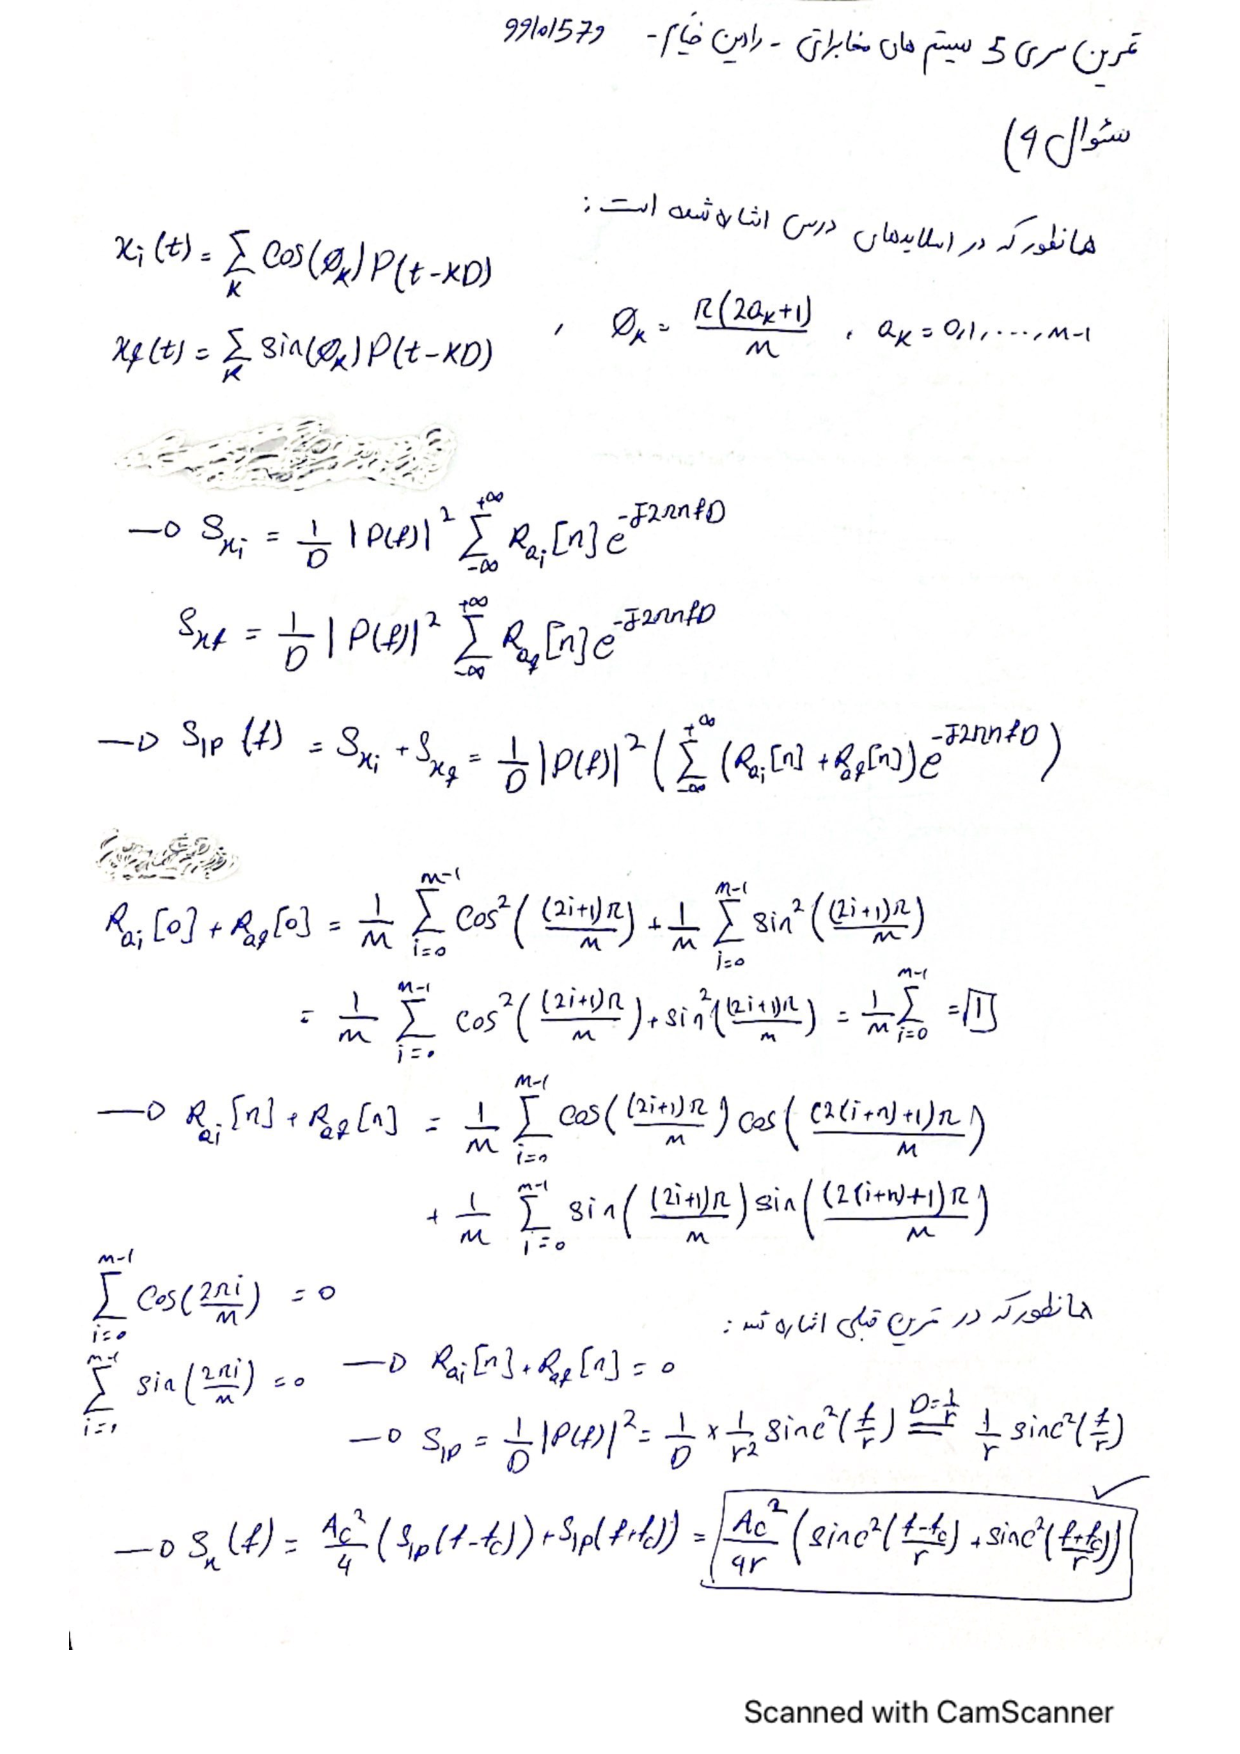
\includegraphics[scale=1]{Fig/Q4.pdf}
\caption{Server and Client.}\label{fig:Q4}
\end{figure}

\begin{subquestion}{Suppose the server is connected to the client with a copper cable, and the transmission loss of the line is $2$ dB/km. Is it possible to have a successful connection without using any amplifier?}
\answer{
$P_{T}=125mW \rightarrow P_{R}=\frac{P_{T}}{10^{\frac{200 \times 2}{10}}}= \frac{125 \times 10^{-3}}{10^{40}}=125 \times 10^{-43}W$\\~\\
$(\frac{S}{N})_{o}=\frac{P_{R}}{N_{0}W}=\frac{125 \times 10^{-43}}{4 \times 10^{-21} \times 400KHz} = \frac{125 \times 10^{-43}}{16 \times 10^{-16}} \cong 7.8 \times 10^{-27} \cong \boxed{-261\,dB}$\\~\\
As we can see the SNR in this condition is equal to -261dB which is less than the minimum acceptable SNR(30 dB), so it is not possible to have a successful connection.
}
\end{subquestion}

\begin{subquestion}{Assume that we have $m$ identical amplifiers, each with a gain of 10 dB. If your answer to the last part is no, find the minimum of $m$ to have a successful connection.}
\answer{
$P_{R}=\frac{P_{T} \times 10^{m}}{10^{40}}=\frac{125 \times 10^{-3+m}}{10^{40}} = 125 \times 10^{m-43}\,W$\\~\\
$(\frac{S}{N})_{o}=\frac{P_{R}}{N_{0}W}=\frac{125 \times 10^{m-43}}{16 \times 10^{-16}}  \cong 7.8 \times 10^{m-27} \cong \left(-261  + 10m \right) $\\~\\
in order to have a successful connection the SNR must be larger than 30dB so:\\~\\
$10m > 261+30 \rightarrow m > 29.1 \rightarrow \textbf{ \boxed{m_{min}=30}}$
}
\end{subquestion}

\begin{subquestion}{Repeat the previous parts assuming the server and the client are connected with an optical fiber, and the transmission loss of the line is $0.3$ dB/km.}
\answer{
$P_{R}=\frac{P_{T}}{10^{\frac{200 \times 0.3}{10}}}= \frac{125 \times 10^{-3}}{10^{6}}=125 \times 10^{-9}W$\\~\\
$(\frac{S}{N})_{o}=\frac{P_{R}}{N_{0}W}=\frac{125 \times 10^{-9}}{4 \times 10^{-21} \times 400KHz} = \frac{125 \times 10^{-9}}{16 \times 10^{-16}} \cong 7.8 \times 10^{+7} \cong \boxed{+78.9\,dB}$\\~\\
so with the optical fiber, the SNR is equal to +78.9\,dB which is larger than +30\,dB hence we have a successful connection without using any amplifier.
}
\end{subquestion}
\end{question}


%----------------------------------------------------------------------------------------
%	QUESTION 5
%----------------------------------------------------------------------------------------

\begin{question}
\questiontext{Fig. \ref{fig:Q5} shows the schematic of a ring modulator.
}
\begin{figure}[H]
\centering
\includegraphics[scale=1]{Fig/Q5.pdf}
\caption{Ring modulator.}\label{fig:Q5}
\end{figure}

\begin{subquestion}{Show that if $|m(t)|\ll 1$, then $u(t)$ is a DSB-modulated signal.}
\answer{ if $|m(t)|\ll 1$ it means that the amplitude of m(t) is much smaller than the amplitude of s(t) so we can assume diodes are switched ON  and OFF by the carrier signal . as we can see if s(t) is equal to 1 two horizontal diodes are switched on and other two diodes are off, so the output signal is equal to m(t). then if s(t) is equal to -1, not horizontal diodes are switched on and the other two diodes become off, so the output signal will be equal to -m(t) so we have these two states so far: \\
\begin{equation*}
v_{o}(t) = \begin{cases}
m(t) & \quad s(t) \ge 0 \\
-m(t) & \quad s(t) \le  0
\end{cases}
\quad \rightarrow \quad v_{o}(t) = m(t)s(t)\\
\end{equation*}
now we put the Fourier series of s(t) instead of itself:
$$v_{o}(t)=m(t)\frac{4}{\pi}\sum_{n=-1}^\infty \frac{(-1)^{n-1}}{2n-1} cos(2\pi f_{c}(2n-1)t)$$
now if we pass $v_{o}(t)$ through a bandpass filter with the center frequency $f = f_{c}$ and the bandwidth 2W we will have:\\
$$v_{o}(t)=\frac{4}{\pi}m(t)cos(2\pi f_{c}t)$$
and finally, we have a signal in the format of $A_{c}m(t)cos(2\pi f_{c}t)$ so we can conclude that the output is a DSB-modulated signal.
}
\end{subquestion}

\begin{subquestion}{What are the main roles of the three-winding transformers in the ring modulator?}
\answer{
we use these transformers to isolate the input from other parts of the circuit and we can remove the DC part of m(t) with them. also, we can easily negate the signal which is useful in some applications. 
}
\end{subquestion}

\end{question}

%----------------------------------------------------------------------------------------
%	QUESTION 6
%----------------------------------------------------------------------------------------

\begin{question}
\questiontext{An SSB-modulated signal having the bandwidth $W$ and power $P_m$ passes through a distortion-less channel with the attenuation $A$ and delay $D$, as shown in Fig. \ref{fig:Q6}.
}
\begin{figure}[h]
\centering
\includegraphics[scale=0.75]{Fig/Q6.pdf}
\caption{Block diagram of an SSB communication system.}\label{fig:Q6}
\end{figure}

\begin{subquestion}{Find the power of the detected signal $\tilde{m}(t)$.}
\answer{
\[  u(t)=A_{c}m(t)\cos(2\pi f_{c}t) \]
\[\rightarrow  k(t)=A_{c}m(t)\cos(2\pi f_{c}t) \mp A_{c}\hat{m}(t)\sin(2\pi f_{c}t)  \]
\[\rightarrow  c(t)=Ak(t-D)=AA_{c}m(t-D)\cos(2\pi f_{c}(t-D)) \mp AA_{c}\hat{m}(t-D)\sin(2\pi f_{c}(t-D))  \]
\[\rightarrow  r(t)=c(t)  \]
\[\rightarrow  v(t)=A_{l}r(t)\cos(2\pi f_{c}t+\phi) \]
\[=  \frac{AA_{l}A_{c}}{2}\big(m(t-D)\cos(2\pi f_{c}t)\cos(2\pi f_{c}t+\phi) \mp \hat{m}(t-D)\sin(2\pi f_{c}(t-D))\cos(2\pi f_{c}t +\phi)\big) \]
\[=  \frac{AA_{l}A_{c}}{2}\big(m(t-D)\cos(4\pi f_{c}t-2\pi f_{c}D+\phi)+m(t-D)\cos(-2\pi f_{c}D-\phi) \]
\[ \mp \hat{m}(t-D)\sin(4\pi f_{c}t-2\pi f_{c}D+\phi)+\hat{m}(t-D)\sin(-2\pi f_{c}D-\phi)\big) \]
\[\rightarrow \tilde{m}(t) = \frac{AA_{c}A_{l}}{2}\big(m(t-D)\cos(-2\pi f_{c}D-\phi) \mp \hat{m}(t-D)\sin(-2\pi f_{c}D-\phi)\big) \]
\[\rightarrow P_{\tilde{m}}= \lim_{T \to \infty} \frac{1}{T} \int_{-\frac{T}{2}}^{+\frac{T}{2}} |\tilde{m}(t)|^2 \,dt \]
\[ = \lim_{T \to \infty} \frac{A^{2}A_{c}^{2}A_{l}^{2}}{4T} \int_{-\frac{T}{2}}^{+\frac{T}{2}} \big[m^{2}(t-D)\cos^{2}(-2\pi f_{c}D-\phi) + \hat{m}^{2}(t-D)\sin^{2}(-2\pi f_{c}D-\phi) \big]\, dt \]
\[ \mp  \lim_{T \to \infty} \frac{A^{2}A_{c}^{2}A_{l}^{2}}{4T} \int_{-\frac{T}{2}}^{+\frac{T}{2}} \big[2m(t-D)\hat{m}(t-D)\sin(-2\pi f_{c}D - \phi)\cos(-2\pi f_{c}D - \phi)\big]\, dt \]
The first part of the integral is equal to $P_{m}$ and for the second part of the integral we have:
\[ =\lim_{T \to \infty} \frac{A^{2}A_{c}^{2}A_{l}^{2}}{4T} \int_{-\frac{T}{2}}^{+\frac{T}{2}} \big[m(t-D)\hat{m}(t-D)\sin(-4\pi f_{c}D - 2\phi)\big]\, dt \   \]
In question 1 we proved this integral is equal to zero.
\[\rightarrow \boxed{  P_{\tilde{m}}=\frac{A^{2}A_{c}^{2}A_{l}^{2}}{4}P_{m}} \]
}
\end{subquestion}

\begin{subquestion}{Find the power of the signal part in the detected signal $\tilde{m}(t)$.}
\answer{
\[ \tilde{m}(t) = \frac{AA_{c}A_{l}}{2}\big(m(t-D)\cos(-2\pi f_{c}D-\phi) \mp \hat{m}(t-D)\sin(-2\pi f_{c}D-\phi)\big) \]
Now we separate the signal part of $\tilde{m}(t)$:
\[ \rightarrow \frac{AA_{c}A_{l}}{2}m(t-D)\cos(-2\pi f_{c}D-\phi)  \]
\[ \rightarrow P = \lim_{T \to \infty} \frac{A^{2}A_{c}^{2}A_{l}^{2}}{4T} \int_{-\frac{T}{2}}^{+\frac{T}{2}}m^{2}(t-D)\cos^{2}(-2\pi f_{c}D-\phi) \,dt \]
\[ \rightarrow \boxed{ P = \frac{A^{2}A_{c}^{2}A_{l}^{2}}{4}\cos^{2}(-2\pi f_{c}D-\phi) P_{m}}  \]

}
\end{subquestion}


\begin{subquestion}{Calculate the value of the phase shift $\phi$ resulting in the maximum power of the signal part in the detected signal $\tilde{m}(t)$.}
\answer{
\[ \cos(-2\pi f_{c}D-\phi) = 1 \quad \rightarrow \quad -2\pi f_{c}D-\phi=0 \quad \rightarrow \quad \boxed{\phi = -2\pi f_{c}D}   \]
}
\end{subquestion}

\end{question}
%----------------------------------------------------------------------------------------

\assignmentSection{Software Questions}

%----------------------------------------------------------------------------------------
%	QUESTION 6
%----------------------------------------------------------------------------------------
\begin{question}

\questiontext{Develop a MATLAB/Python code that accepts the message signal $m(t)$ and generates time- and frequency-domain plots of the corresponding DSB-, LSSB-, USSB-, and AM-modulated signals. The input arguments of the function are message signal $m(t)$, carrier frequency $f_c$, carrier amplitude $A_c$, AM modulation index $a$, and modulation type. Investigate the outputs of the function for a sample message signal.
}

\answer{
There is a Matlab file named Q7 in the zip file. 
We assume $m(t)=cos(2\pi f_{m}t)$ and then calculate the DSB, USSB, LSSB, and AM modulation of this signal.
\pagebreak
DSB Modulating:
\begin{figure}[H]
  \includegraphics[width=\linewidth]{fig/9.jpg}
\end{figure}

\begin{figure}[H]
  \includegraphics[width=\linewidth]{fig/1.jpg}
\end{figure}

\begin{figure}[H]
  \includegraphics[width=\linewidth]{fig/2.jpg}
\end{figure}
\pagebreak
SSB Modulating:
\begin{figure}[H]
  \includegraphics[width=\linewidth]{fig/10.jpg}
\end{figure}

\begin{figure}[H]
  \includegraphics[width=\linewidth]{fig/3.jpg}
\end{figure}

\begin{figure}[H]
  \includegraphics[width=\linewidth]{fig/4.jpg}
\end{figure}

\begin{figure}[H]
  \includegraphics[width=\linewidth]{fig/5.jpg}
\end{figure}

\begin{figure}[H]
  \includegraphics[width=\linewidth]{fig/6.jpg}
\end{figure}
\pagebreak
AM Modulating:
\begin{figure}[H]
  \includegraphics[width=\linewidth]{fig/11.jpg}
\end{figure}

\begin{figure}[H]
  \includegraphics[width=\linewidth]{fig/7.jpg}
\end{figure}

\begin{figure}[H]
  \includegraphics[width=\linewidth]{fig/8.jpg}
\end{figure}
}

\end{question}

%----------------------------------------------------------------------------------------

\assignmentSection{Bonus Questions}

%----------------------------------------------------------------------------------------
%	QUESTION 2
%----------------------------------------------------------------------------------------
\begin{question}
\questiontext{Prove that the time duration $\sigma_t$ and spectral bandwidth $\sigma_f$ satisfy the inequality $$\sigma_t \sigma_f \geqslant \frac{1}{4\pi}$$, where the time duration
$$
\sigma_t^2 = \frac{\int_{-\infty}^\infty (t-\bar{t})^2|x(t)|^2dt}{\int_{-\infty}^\infty |x(t)|^2dt}, \quad \bar{t}=\frac{\int_{-\infty}^\infty t|x(t)|^2dt}{\int_{-\infty}^\infty |x(t)|^2dt}
$$
and the spectral bandwidth
$$
\sigma_f^2 = \frac{\int_{-\infty}^\infty (f-\bar{f})^2|X(f)|^2df}{\int_{-\infty}^\infty |X(f)|^2df}, \quad \bar{f}=\frac{\int_{-\infty}^\infty f|X(f)|^2df}{\int_{-\infty}^\infty |X(f)|^2df}
$$
such that $X(f)=\int_{-\infty}^\infty x(t)e^{-j2\pi f t}dt$. For which signal does the equality hold? Can you provide an intuition for this inequality?
}

\answer{}
\end{question}

%----------------------------------------------------------------------------------------
%	QUESTION 7
%----------------------------------------------------------------------------------------

\begin{question}

\questiontext{Return your answers by filling the \LaTeX template of the assignment.}

\end{question}

%----------------------------------------------------------------------------------------

\end{document}
